%%% Local Variables:
%%% mode: latex
%%% TeX-master: t
%%% End:


%%% Template originaly created by Karol Kozioł (mail@karol-koziol.net) and modified for ShareLaTeX use

\documentclass[a4paper,11pt]{abntex2}

\usepackage[T1]{fontenc}
\usepackage[utf8]{inputenc}
\usepackage{graphicx}
\usepackage{xcolor}

\renewcommand\familydefault{\sfdefault}
\usepackage{tgheros}
% \usepackage{Consolatas}
\usepackage{yfonts}

\usepackage{amsmath,amssymb,amsthm,textcomp}
% \usepackage[noitemsep]{enumerate}
% \setlist{noitemsep}
% \selist{nosep}

\setlist[2]{noitemsep} % sets the itemsep and parsep for all level two lists to 0

\setenumerate{noitemsep} % sets no itemsep for enumerate lists only
\begin{enumerate}[noitemsep] % sets no itemsep for just this list
  % ...
\end{enumerate}


\usepackage{multicol}
\usepackage{tikz}

\usepackage[margin=1in]{geometry}
\geometry{left=25mm,right=25mm,%
  bindingoffset=0mm, top=20mm,bottom=20mm}


\linespread{1.1}

\newcommand{\linia}{\rule{\linewidth}{0.5pt}}

% custom theorems if needed
\newtheoremstyle{mytheor}
{1ex}{1ex}{\normalfont}{0pt}{\scshape}{.}{1ex}
{{\thmname{#1 }}{\thmnumber{#2}}{\thmnote{ (#3)}}}

\theoremstyle{mytheor}
\newtheorem{defi}{Definition}

% my own titles
\makeatletter
\renewcommand{\maketitle}{
  \begin{center}
    \vspace{4ex}
    { {\fontsize{40}{40}\selectfont \textfrak{\@title}} }
    \vspace{2ex}
    \\
    \linia\\
    \@author \hfill \@date
    \vspace{6ex}
  \end{center}
}
\makeatother
%%%

% custom footers and headers
\usepackage{fancyhdr}
\pagestyle{fancy}
\lhead{}
\chead{}
\rhead{Entrega até 14/05}
\lfoot{Lista \textnumero{} 1}
\cfoot{}
\rfoot{Página \thepage}
\renewcommand{\headrulewidth}{0.5pt}
\renewcommand{\footrulewidth}{0.5pt}
%

%%% ----------%%%----------%%%----------%%%----------%%%

\usepackage{hyperref}

{%Muda a cor do Sumário, pois são todo links.
  \hypersetup{
    colorlinks=true,
    citecolor= violet,
    linkcolor=black!85,
    filecolor=magenta,
    urlcolor=cyan,
  }

  %%% ----------%%%----------%%%----------%%%----------%%%

  \begin{document}

  \title{Lis:ta 1}

  \author{\indent  Prof.: Pedro G. Branquinho, EEL-USP. \\
    Orient.: Katia C. G. Candioto.}

  \date{06/05/20 - 13/05/20}

  \maketitle

  \section*{Problema 1}

  Utilizando o template, no repositório do
  \href{https://github.com/26-55-87-BuddhiLW/MC-LaTeX/tree/master/Exemplos/ArquivosCurso/ModRelatCient}{GitHub},
  \textbf{(re)produza uma capa e folha de capa}, com um título de pesquisa que gostaria de fazer
  pra um possível TCC (o assunto pode ser, por exemplo, culinária; ou
  sistemas dinâmicas).  O modelo deve estar de acordo com as
  seguintes normas, ABNT,

  \begin{itemize}[noitemsep]

  \item NBR 6023, Informação e documentação: referências: elaboração.
  \item NBR 6024, Informação e documentação: numeração progressiva das seções de um documento escrito: apresentação.
  \item NBR 6027, Informação e documentação: sumário: apresentação.
  \item NBR 6028, Informação e documentação: resumo: apresentação.
  \item NBR 10520, Informação e documentação: citações em documentos:apresentação.
  \item NBR 12225, Informação e documentação: lombada: apresentação.
  \item NBR 14724, Informação e documentação: trabalhos acadêmicos: apresentação.

  \end{itemize}

  Como prescrito na diretriz, no site da
  \href{http://sistemas.eel.usp.br/bibliotecas/arq/diretrizes_usp_eel_2009!.pdf}{EEL-USP}. Mais
  especificamente,

  A capa, em ordem, deve conter,

  \begin{enumerate}
    \noitemsep
  \item nome da instituição (opcional);
  \item nome completo do autor;
  \item título: em letras minúsculas, com exceção da primeira letra,
    nomes próprios ou científicos;
  \item subtítulos (se houver);
  \item número de volumes (se houver mais de um);
  \item local (cidade);
  \item  ano de depósito (da entrega).
  \end{enumerate}

  A folha de rosto, por sua vez, deve conter, como itens essenciais,

  \begin{enumerate}
  \item  nome completo do autor;
  \item  título;
  \item  subtítulo (se houver);
  \item  número de volumes (se houver mais de um);
  \item  natureza do trabalho (dissertação ou tese);
  \item nome da instituição a que é submetido o trabalho;
  \item  grau pretendido (aprovação em disciplina);
  \item área de concentração;
  \item  nome do orientador, co-orientador2 (se houver);
  \item  local (cidade);
  \item  ano de depósito (da entrega).
  \end{enumerate}

  \clearpage
  Os exemplos dados na diretriz da EEL-USP, fornece os seguintes
  exemplos,

  \begin{figure}[!htb]
    \begin{center}
      \caption{\label{fig:cp} Capa}\\

      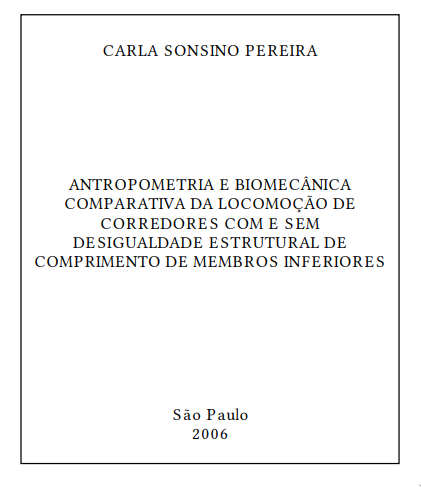
\includegraphics[scale=0.5]{./imagens/2.png} \\

      \legend{Fonte: \href{http://sistemas.eel.usp.br/bibliotecas/arq/diretrizes_usp_eel_2009!.pdf}{diretrizes EEL-USP}}
    \end{center}
  \end{figure}

  \begin{figure}[!htb]
    \begin{center}
      \caption{\label{fig:fr} Folha de Rosto}\\

      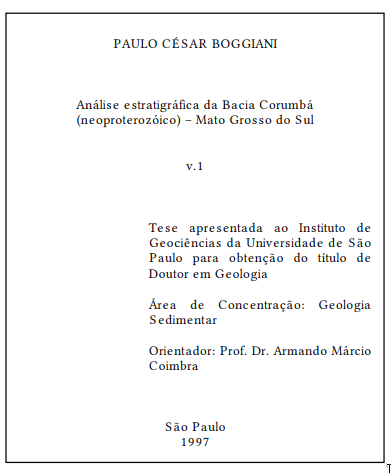
\includegraphics[scale=0.5]{./imagens/1.png}\\

      \legend{Fonte: \href{http://sistemas.eel.usp.br/bibliotecas/arq/diretrizes_usp_eel_2009!.pdf}{diretrizes EEL-USP}}
    \end{center}
  \end{figure}

  \begin{center}
  {\noindent \textcolor{red!70!black}{ \textbf{(Obs: O problema é mais simples
      do que parece à primeira vista. Perceba que a classe abntex2,
      utilizada no
      \href{http://sistemas.eel.usp.br/bibliotecas/arq/diretrizes_usp_eel_2009!.pdf}{modelo}
      está de acordo com as normas ABNT. Com pequenos modificações,
      fica-se semelhante aos modelos na diretriz da EEL-USP.)}}}}
\end{center}

\clearpage



\section*{Problem 2}

\textbf{2.(a) Reescreva a seguinte fórmula,}

\begin{figure}[!htb]
  \begin{center}
    \caption{\label{fig:ForLatex} } Fórmula em \TeX \\

    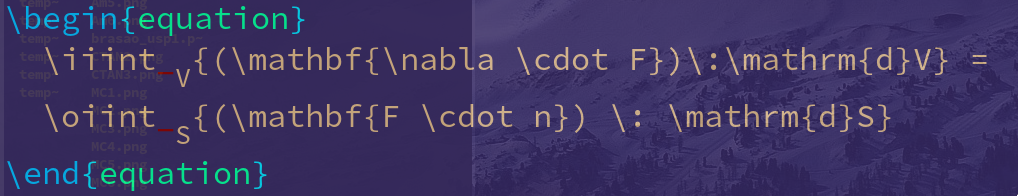
\includegraphics[scale=0.5]{./imagens/A2I71.png}\\

    \legend{Fonte: o autor}
  \end{center}
\end{figure}

\begin{figure}[!htb]
  \begin{center}
    \caption{\label{fig:mapa} Resultado}\\

    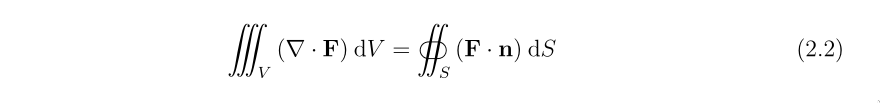
\includegraphics[scale=0.5]{./imagens/A2I72.png}\\

    \legend{Fonte: o autor}
  \end{center}
\end{figure}

\textcolor{red!70!black}{\textbf{(Obs: não é para ter o numeral (2.2) ao lado direito, como na imagem).}}

\vspace{0.5cm}
{\noident\textbf{2.(b) Em seguida, escreva a seguinte fórmula,}}

\begin{equation}
  \int_{- \infty}^{\infty}{e^{-x^2} \mathrm{d}x}=1
\end{equation}

\clearpage

\section*{Problema 3}

\textbf{Reproduza o seguinte ambiente de itemização}. Modifique-o,
colocando um(diversos)
símbolo(s) nos itens (o texto é irrelevante). Os itens  \textbf{não}
devem ser idênticos aos da imagem, mas pode-se(use!) utilizar o mesmo pacote
(digbat) utilizado para gerar a itemização da imagem. \href{https://github.com/26-55-87-BuddhiLW/MC-LaTeX/tree/master/Exemplos/ArquivosCurso/ModApresent}{No
  modelo de aprensetação}, se encontra tudo necessário para a
reprodução requisitada.

\begin{figure}[!htb]
  \begin{center}
    \caption{\label{fig:itemizacao} Itemização estilizada, modelo de
      itemização 1}\\

    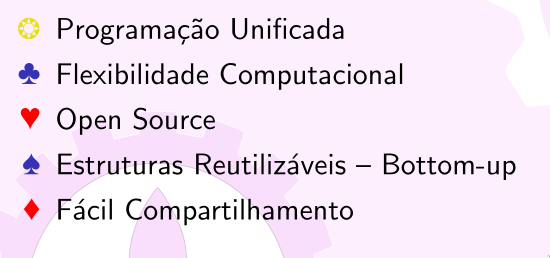
\includegraphics[scale=0.5]{./imagens/3.png}\\

    \legend{Fonte: o autor}
  \end{center}
\end{figure}

\begin{figure}[!htb]
  \begin{center}
    \caption{\label{fig:itemizacao} Itemização estilizada, modelo de
      itemização 2}\\

    
\includegraphics[scale=0.5]{./imagens/4.png}\\

    \legend{Fonte: o autor}
  \end{center}
\end{figure}




\end{document}

%%% Local Variables:
%%% mode: latex
%%% TeX-master: t
%%% End:
